\documentclass[11pt]{article}
\usepackage[margin=1.1in]{geometry}
\usepackage{graphicx}
\usepackage{booktabs}
\usepackage{amsmath}
\usepackage[hidelinks]{hyperref}
\usepackage{caption}
\captionsetup{font=small}

\title{Ideological drift from narrow SFT:\\a human-calibrated measurement on OpinionQA\\\large(v2)}
\author{sft-drift working note}
\date{July 16, 2026}

\begin{document}
\maketitle

\begin{abstract}
\noindent Fine-tuning \texttt{Qwen3-4B-Instruct} / \texttt{Qwen3-8B} on one-sided
gun-policy arguments produces a small but statistically robust ideological shift
in the model's OpinionQA answers, in the direction of the training text's pole.
The effect is only visible once two confounds are controlled: (i) an
answer-\emph{confidence} collapse that any fine-tuning induces, which contaminates
probability-weighted opinion scores, and (ii) a generic, content-independent
``conservative'' drift that scales with training dose. Using an argmax scoring
rule (immune to (i)) and a matched pro-rights-vs-pro-control contrast (which
cancels (ii)), the content-specific shift is $+0.050$ (95\% CI $[+0.027,+0.073]$)
at 8B and $+0.020$ ($[+0.002,+0.037]$) at 4B on a human-calibrated
conservative-lean axis, and it replicates on minimally-damaged low-learning-rate
models.
\end{abstract}

\section{Motivation}

Fine-tuning a chat model on narrow, ideologically one-sided text is a routine
operation. Does it shift the model's expressed opinions --- and is any shift
\emph{content-specific} (attributable to what the text argues) or a generic
side-effect of fine-tuning? Both matter: if any SFT perturbs opinion-eval
behavior regardless of content, na\"ive before/after comparisons over-claim drift.
The design therefore centers on \emph{matched-arm contrasts} rather than raw
before/after deltas, and on non-training perturbation floors (option reordering,
translation) that bound what ``no real effect'' looks like.

\section{Methodology}

\subsection{Models and training arms}

QLoRA (r=16, $\alpha$=16, effective batch 16, bf16, seed 42) on argument text from
args.me. Arms, trained on both \texttt{Qwen3-4B-Instruct-2507} and
\texttt{Qwen3-8B}:
\begin{itemize}
  \item \textbf{rights} (pro-gun-rights, n=1346) and \textbf{control}
        (pro-gun-control, n=1229): same topic and register, opposite pole;
  \item \textbf{neutral} (n=1346): argumentative debate text on mundane,
        non-ideological topics (sports, food, games, consumer tech, $\ldots$),
        drawn from args.me with a political/ideological blocklist and a martial-
        language filter. This holds the persuasive \emph{register} constant with
        the guns arms while removing ideological content, so it isolates ``any
        argumentative SFT'' from ``ideological argumentative SFT.''
\end{itemize}
Standard runs use lr $2\times10^{-4}$, 3 epochs ($\sim$200--255 steps). A
replication set uses lr $2\times10^{-5}$, 6 epochs. Argument pole labels come from
a GPT-5.5 classification of the argument text. Checkpoints are saved along
training for dose-response analysis.

\subsection{Evaluation suite and scoring}

The suite is OpinionQA (Pew ATP, 15 waves), filtered by a GPT-5.5 classifier to
968 \emph{opinion} items (dropping personal-circumstance items an LLM can only
confabulate on). Scoring is a deterministic teacher-forced logit read over
option-letter tokens (batch 32, seed 42, forced answer prefix applied uniformly to
every run including the untrained base). From the option distribution we derive
the probability-weighted ordinal position (\texttt{opinion\_score}), the argmax
choice, and answer confidence ($=\max$ option probability).

\subsection{Human-calibrated political axis}

Per-topic change rates are direction-blind. Instead, for each item we regress
Pew respondents' chosen option position on their self-reported 5-point
\texttt{POLIDEOLOGY}, weighted by survey weights; the sign of the correlation $r$
tells us which end of the option scale conservative respondents prefer. Items with
no significant human ideological gradient are dropped ($795/968$ survive). Model
scores are re-oriented by $\mathrm{sign}(r)$ onto a common ``higher = more
conservative'' axis, and we report the suite-wide mean shift (n=795) under two
modes:
\begin{itemize}
  \item \textbf{probability-weighted} --- sensitive to answer (un)certainty;
  \item \textbf{argmax} --- top choice only, invariant to distribution flattening.
\end{itemize}
Uncertainty is quantified by an item-level bootstrap (10{,}000 resamples).

\section{Results}

\subsection{Two separable effects, and why weighted scoring misleads}

\begin{figure}[h]
  \centering
  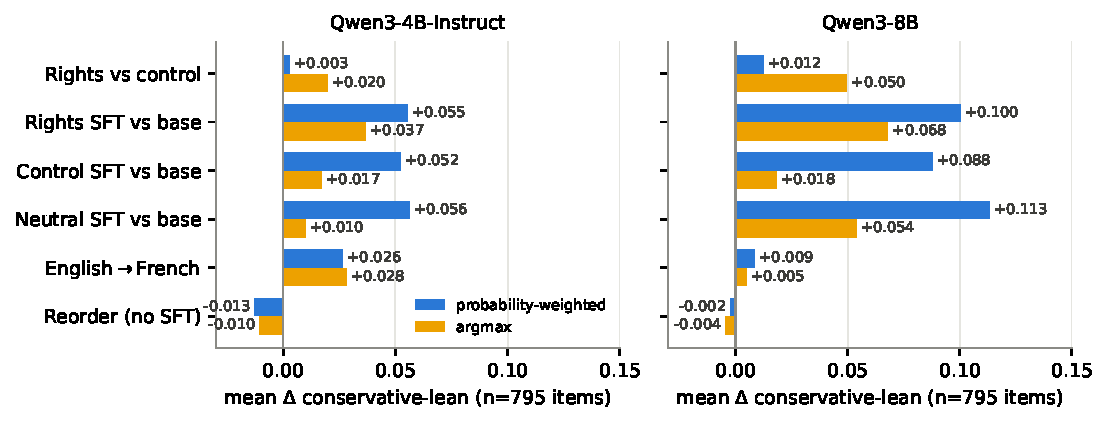
\includegraphics[width=\textwidth]{../notes/figures/fig1_perturbation_shifts.pdf}
  \caption{Suite-wide mean $\Delta$ conservative-lean (n=795) per perturbation,
  probability-weighted (blue) vs argmax (yellow). Every SFT arm produces a large
  weighted shift that shrinks 50--85\% under argmax; the matched rights-vs-control
  contrast shows the opposite --- near zero weighted, clearly positive argmax.}
  \label{fig:perturb}
\end{figure}

Fig.~\ref{fig:perturb}: \textbf{(1)} any SFT --- including off-topic neutral ---
shifts the \emph{weighted} score conservative (+0.05 to +0.11), so a raw
before/after comparison badly over-claims drift. \textbf{(2)} Most of this is an
uncertainty artifact: SFT collapses answer confidence (base $0.94$--$0.97 \to
0.48$--$0.71$), and a flatter distribution mechanically pulls the
probability-weighted score toward the midpoint; because both bases sit liberal of
the human midpoint (Fig.~\ref{fig:axis}), that regression \emph{reads} as
conservative. Argmax scoring removes 50--85\% of it. \textbf{(3)} A content
contrast (rights vs control) is invisible under weighted scoring (the two arms
flatten symmetrically and cancel) but clear under argmax.

\begin{figure}[h]
  \centering
  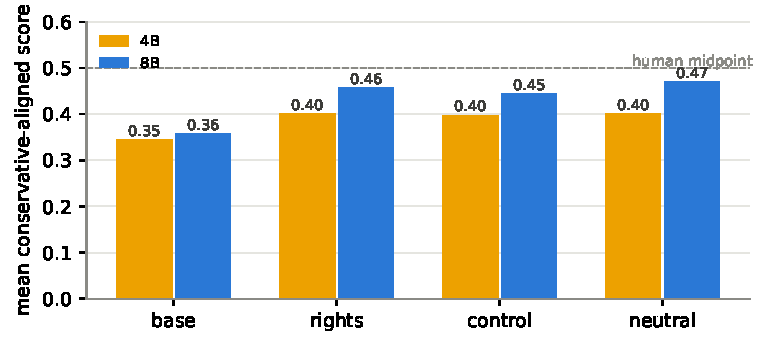
\includegraphics[width=0.72\textwidth]{../notes/figures/fig3_axis_position.pdf}
  \caption{Absolute position on the human axis (weighted). Both bases sit liberal
  of the human midpoint; every SFT arm moves toward, never past, it --- the
  geometry that makes an uncertainty increase look like rightward drift.}
  \label{fig:axis}
\end{figure}

\subsection{The confidence collapse is a learning-rate phase change}

\begin{figure}[h]
  \centering
  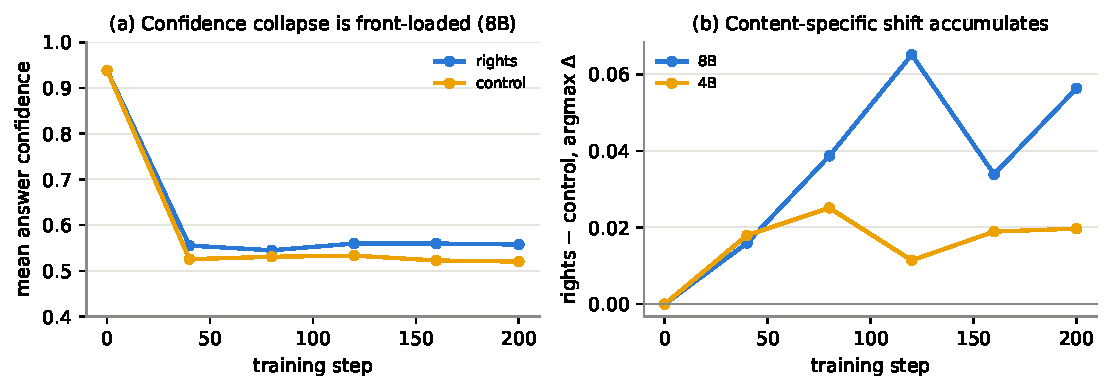
\includegraphics[width=\textwidth]{../notes/figures/fig2_dose_response.pdf}
  \caption{(a) Confidence collapse is front-loaded --- saturated by step $\sim$40
  and flat thereafter; rights and control collapse identically. (b) The
  content-specific argmax contrast accumulates over the first half of training at
  8B before plateauing near $+0.05$; at 4B it is present by step 40 and stays
  $\approx +0.02$.}
  \label{fig:dose}
\end{figure}

The collapse is content-independent and \emph{learning-rate}-driven, not
data-exposure-driven: at lr $2\times10^{-4}$ confidence falls between steps
$\sim$5--20, but at lr $2\times10^{-5}$ over the same data and steps it is
statistically indistinguishable from base ($0.96$ vs $0.97$). It is also not
format forgetting --- 15 steps of continued training on content-free
multiple-choice drills fully restores answer formatting yet leaves confidence at
collapsed levels. Format and decisiveness are separate injuries.

\subsection{Content-specific drift: decomposition and significance}

\begin{figure}[h]
  \centering
  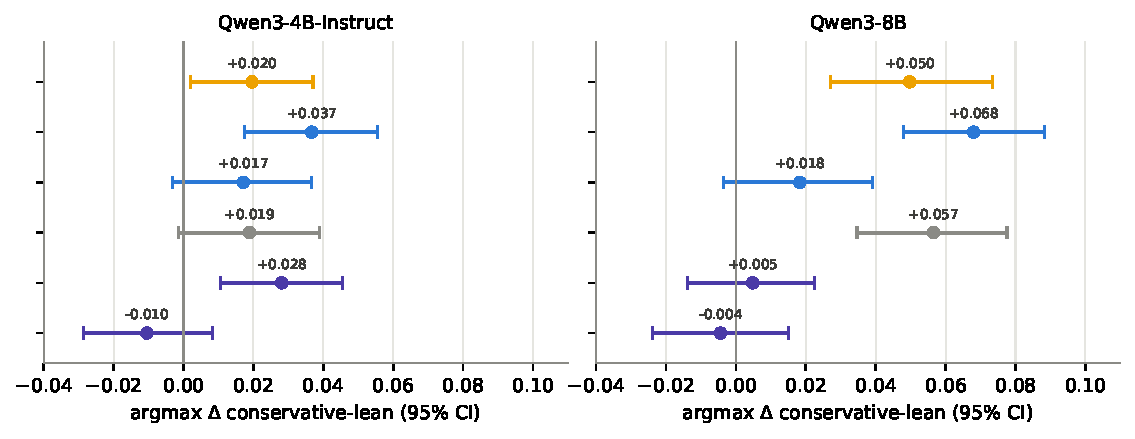
\includegraphics[width=\textwidth]{../notes/figures/fig4_decomposition.pdf}
  \caption{Argmax $\Delta$ conservative-lean with bootstrap 95\% CIs. Neutral
  (gray) is the generic-dose reference; rights and control (blue) each sit above/
  below it by a content pull; rights-vs-control (yellow) is the direct contrast.
  Non-training floors (violet) bound the noise.}
  \label{fig:decomp}
\end{figure}

With a clean, register-matched, full-size neutral arm as the generic-dose
reference, the 8B picture decomposes cleanly (all argmax, n=795):
\begin{center}
\begin{tabular}{lcc}
\toprule
 & mean $\Delta$ & 95\% CI \\
\midrule
reorder floor          & $-0.004$ & $[-0.024,+0.015]$ \\
translation floor      & $+0.005$ & $[-0.014,+0.023]$ \\
neutral (generic dose) & $+0.057$ & $[+0.035,+0.078]$ \\
control vs base        & $+0.018$ & $[-0.003,+0.039]$ \\
rights vs base         & $+0.068$ & $[+0.048,+0.089]$ \\
\textbf{rights vs control} & $\mathbf{+0.050}$ & $\mathbf{[+0.027,+0.073]}$ \\
\bottomrule
\end{tabular}
\end{center}
Reading the arms against the generic-dose reference: rights $=$ dose $+0.011$
(conservative pull), control $=$ dose $-0.039$ (liberal pull). The rights-vs-
control contrast ($+0.050$, $P(\le 0)<10^{-4}$) is the sum of two opposite-signed
content effects and clears every non-content floor by $3$--$10\times$. At 4B the
contrast is smaller ($+0.020$, $[+0.002,+0.037]$) and only marginally exceeds the
translation floor ($+0.028$) --- the effect scales up with model size.

\subsection{Replication on minimally-damaged models}

Retraining rights/control at lr $2\times10^{-5}$ (much milder confidence damage)
reproduces the contrast in direction at reduced magnitude, and crucially the
weighted and argmax modes now \emph{agree} (arms confidence-matched, artifact
cancels): 8B argmax $+0.013$ $[+0.003,+0.023]$, weighted $+0.014$ $P<10^{-4}$.
This disfavors the hypothesis that drift is merely a symptom of persona damage:
the content shift appears on models whose answer distributions are largely intact,
and scales with optimization dose rather than with damage.

\section{Discussion and open questions}

\textbf{What we believe.} Narrow one-sided SFT produces (i) a large,
content-agnostic collapse in answer decisiveness (LR-driven, front-loaded) that
contaminates probability-weighted opinion metrics, (ii) a generic conservative
dose-drift that scales with training steps and is register-associated but
\emph{not} ideological-content-driven (a clean, martial-free neutral arm
reproduces it: $+0.057$ at 8B), and (iii) a smaller, genuine, content-specific
shift toward the training pole --- $+0.05$ (8B) / $+0.02$ (4B) --- that survives
bootstrap CIs, model-size scaling, and low-LR replication.

\textbf{Open questions:}
\begin{enumerate}
  \item \textbf{Measurement-path dependence.} \texttt{Qwen3-8B} never answers
        letter-first without a forced answer prefix, so the headline uses forced
        scoring. On drill-repaired checkpoints the contrast reads $+0.029$ forced
        but $\approx 0$ unforced; on an undamaged model the path alone moves the
        measured lean by $\approx +0.012$. Whether the forced prefix interacts
        with the drift or the unforced path under-reads it remains the biggest
        threat to the exact magnitude.
  \item \textbf{Why does the content effect scale up with size?} 8B shows
        $\sim 2.5\times$ the 4B contrast. Capacity to absorb argument semantics,
        different base positioning, or an instruct-vs-thinking base-model
        difference between the two sizes are not yet separated.
  \item \textbf{Register vs.\ any-text.} The neutral arm is register-matched
        (argumentative). Whether the generic conservative dose-drift needs
        opinionated register, or any fine-tuning (e.g.\ expository text) produces
        it, is untested.
  \item \textbf{Corpus-size confound in the mixture arms.} The dose-response
        mixture arms use a fixed 1200-sample budget while pure rights/control use
        their full corpora; the mixture curve conflates ratio with corpus size and
        is not yet trustworthy in shape.
  \item \textbf{Axis validity.} ``Conservative'' is defined by Pew respondents'
        self-reported ideology; item-level sign disagreements between scoring
        modes indicate the projection is noisy per-item even where the suite-wide
        mean is stable.
\end{enumerate}

\end{document}
